\documentclass[letterpaper, 11 pt]{article}

\usepackage{fullpage}

\usepackage{algorithmic}
\usepackage{graphics}
\usepackage{epsfig}
\usepackage{subfigure}
\usepackage{stfloats}
\usepackage{wrapfig}
%\title{\bf Proposal: Waypoint a Room with Simple Diff-Drive Robots}

\author{Kevin Kemper}

\begin{document}

\begin{flushright}
Kevin Kemper
\end{flushright}

\vspace{-2cm}
\begin{center}
\textbf{\huge ME537: Homework 2}
\end{center}


\thispagestyle{empty}
\pagestyle{empty}


%1- Precisely describe each algorithm you used and your experimental methodology. Record
%the run time, solution quality and repeatability of each approach (solve the problem at least
%10 times and provide statistical results) and discuss your results for the T10 problem.


\vspace{0.5cm}

For all algorithms and trials: $\epsilon = 0.1$, $\alpha = 0.001$, $\gamma = 0.1$ and
$T = 0.1$


\section{Part 1 - n-Arm bandit}



%\begin{wrapfigure}{r}{0.5\textwidth}
\begin{figure}[htb]
	\centering
	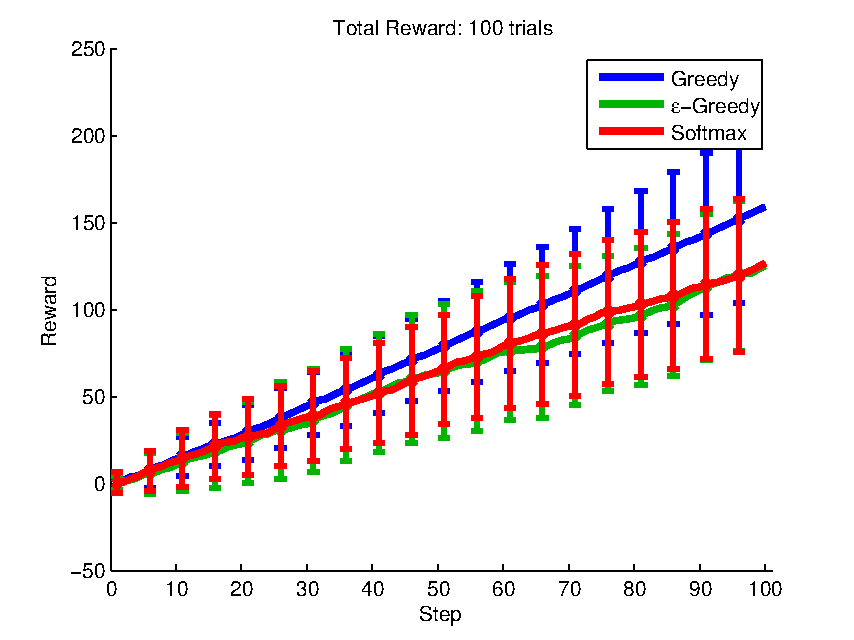
\includegraphics[scale=0.6]{../figures/part1.pdf}
	\caption{\small	Results for thee different action-value functions.  Greedy ends up
						preforming better but the variance is very high for all cases.
			}
	\label{fig:pathsa}
%\end{wrapfigure}
\end{figure}

\begin{figure}[htb]
	\centering
	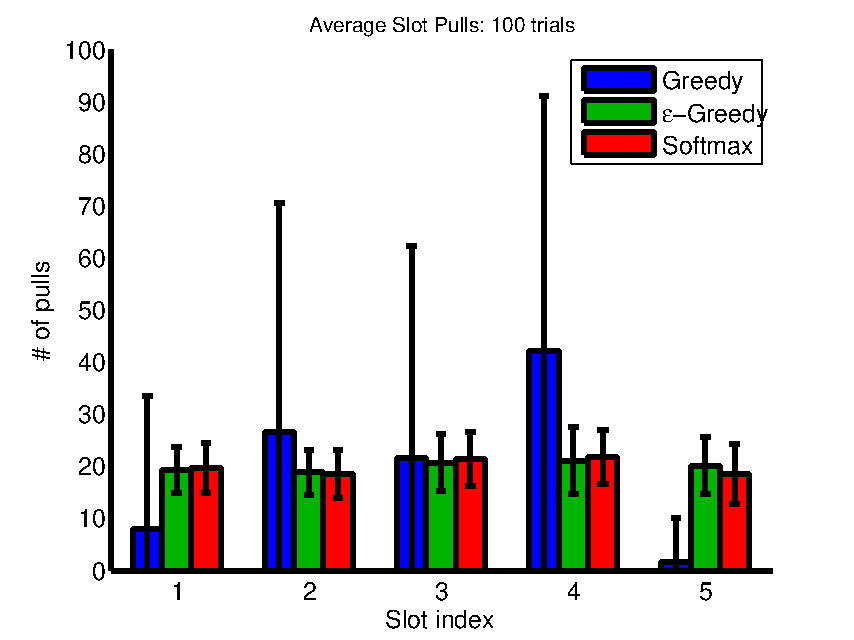
\includegraphics[scale=0.6]{../figures/part1_hits.pdf}
	\caption{\small	Number of slot pulls for the thee different action-value functions.
					Greedy tended to choose slot 4 while the others had even distribution.
			}
	\label{fig:pathsa}
%\end{wrapfigure}
\end{figure}




\pagebreak
\section{Part 2 - Gridworld}



\begin{figure}[htb]
	\centering
	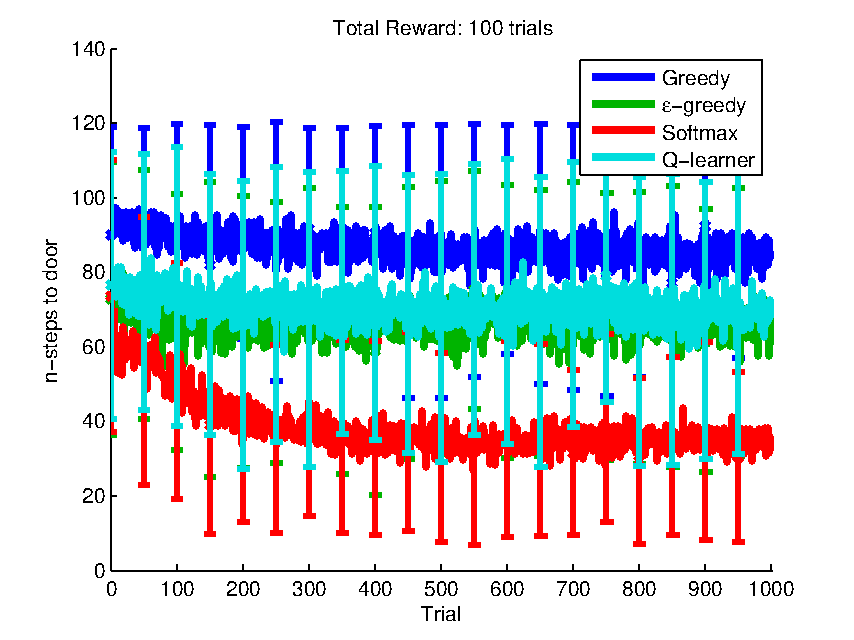
\includegraphics[scale=0.7]{../figures/part2.pdf}
	\caption{\small	Average number of steps to find the goal.  Softmax outperformed
					all the others with $\epsilon$-greedy doing the next best.
			}
	\label{fig:pathsa}
%\end{wrapfigure}
\end{figure}








\end{document}
